\documentclass[UTF8]{ctexart}
\usepackage{amsmath}
\usepackage{graphicx}
\graphicspath{{figure/}}
\usepackage{svg}
\usepackage{fancyhdr}
\usepackage{geometry}
\geometry{left=2cm, right=2cm, top=3cm, bottom=4cm}
\usepackage{setspace}
\onehalfspacing
\usepackage{fancyhdr}
\pagestyle{fancy}
\lhead{\author}
\chead{\date}
\lfoot{}
\cfoot{\thepage}
\rfoot{}
\renewcommand{\headrulewidth}{0.4pt}
\renewcommand{\headwidth}{\textwidth}
\renewcommand{\footrulewidth}{0pt}
% 导言区

\title{德州扑克概率分析}
\author{daniu22}
\date{\today}
\begin{document}
\maketitle
\newpage
\tableofcontents
\newpage
\section{历史}
德州扑克最初起源于20世纪初的德克萨斯州,是由当地的赌徒们创造的一种扑克牌游戏。
它很快就流行开来,随着赌场的兴起,德州扑克也成为了赌场中最受欢迎的游戏之一。
如今,德州扑克已经成为了一项全球性的竞技游戏,在世界各地的扑克比赛中得到了广泛应用。
\section{德州扑克规则介绍}
\subsection{基本规则}
\begin{itemize}
    \item 玩家数量:德州扑克至少需要两名玩家,但通常有2-10名玩家参与。
    \item 牌型大小:德州扑克中的牌型大小,从小到大分别为皇家同花顺、同花顺、四条、葫芦、
    同花、顺子、三条、两对、一对和高牌。
    \item 游戏流程:游戏通常分为四轮,每轮之间有加注、跟注、弃牌和全下等选择。
    \item 胜利规则:游戏的目标是赢得其他所有玩家的筹码,通过组合自己手中的牌和五张公共牌,
    构成最优的五张牌来比较大小。
\end{itemize}
\subsection{牌型图示}
\begin{itemize}
    \item 高牌(High Card):
    \begin{figure}[h]
        \centering
        \includegraphics[width=.19\linewidth]{spade_ace.pdf}
        \includegraphics[width=.19\linewidth]{diamond_k.pdf}
        \includegraphics[width=.19\linewidth]{heart_10.pdf}
        \includegraphics[width=.19\linewidth]{club_4.pdf}
        \includegraphics[width=.19\linewidth]{spade_5.pdf} 
        \caption{\label{fig:high_card}高牌示例}
    \end{figure}
    \item 一对(Pair):
    \begin{figure}[h]
        \centering
        \includegraphics[width=.19\linewidth]{spade_ace.pdf}
        \includegraphics[width=.19\linewidth]{diamond_ace.pdf}
        \includegraphics[width=.19\linewidth]{heart_10.pdf}
        \includegraphics[width=.19\linewidth]{club_4.pdf}
        \includegraphics[width=.19\linewidth]{spade_5.pdf} 
        \caption{\label{fig:pair}一对示例}
    \end{figure}
    \item 两对(Two Pair):
    \begin{figure}[h]
        \centering
        \includegraphics[width=.19\linewidth]{spade_ace.pdf}
        \includegraphics[width=.19\linewidth]{diamond_ace.pdf}
        \includegraphics[width=.19\linewidth]{heart_k.pdf}
        \includegraphics[width=.19\linewidth]{club_k.pdf}
        \includegraphics[width=.19\linewidth]{spade_5.pdf} 
        \caption{\label{fig:two_pair}两对示例}
    \end{figure}
    \item 三条(Three of a Kind):
    \begin{figure}[h]
        \centering
        \includegraphics[width=.19\linewidth]{spade_ace.pdf}
        \includegraphics[width=.19\linewidth]{diamond_ace.pdf}
        \includegraphics[width=.19\linewidth]{heart_ace.pdf}
        \includegraphics[width=.19\linewidth]{club_4.pdf}
        \includegraphics[width=.19\linewidth]{spade_5.pdf} 
        \caption{\label{fig:three_kind}三条示例}
    \end{figure}
    \item 顺子(Straight):
    \begin{figure}[h]
        \centering
        \includegraphics[width=.19\linewidth]{spade_ace.pdf}
        \includegraphics[width=.19\linewidth]{diamond_k.pdf}
        \includegraphics[width=.19\linewidth]{heart_q.pdf}
        \includegraphics[width=.19\linewidth]{club_j.pdf}
        \includegraphics[width=.19\linewidth]{spade_10.pdf} 
        \caption{\label{fig:straight}顺子示例}
    \end{figure}
    \item 同花(Flush):
    \begin{figure}[h]
        \centering
        \includegraphics[width=.19\linewidth]{spade_ace.pdf}
        \includegraphics[width=.19\linewidth]{spade_k.pdf}
        \includegraphics[width=.19\linewidth]{spade_10.pdf}
        \includegraphics[width=.19\linewidth]{spade_4.pdf}
        \includegraphics[width=.19\linewidth]{spade_5.pdf} 
        \caption{\label{fig:flush}同花示例}
    \end{figure}
    \item 葫芦(Full House):
    \begin{figure}[h]
        \centering
        \includegraphics[width=.19\linewidth]{spade_ace.pdf}
        \includegraphics[width=.19\linewidth]{diamond_ace.pdf}
        \includegraphics[width=.19\linewidth]{heart_ace.pdf}
        \includegraphics[width=.19\linewidth]{club_k.pdf}
        \includegraphics[width=.19\linewidth]{spade_k.pdf} 
        \caption{\label{fig:full_house}葫芦示例}
    \end{figure}
    \item 四条(Four of a Kind):
    \begin{figure}[h]
        \centering
        \includegraphics[width=.19\linewidth]{spade_ace.pdf}
        \includegraphics[width=.19\linewidth]{diamond_ace.pdf}
        \includegraphics[width=.19\linewidth]{heart_ace.pdf}
        \includegraphics[width=.19\linewidth]{club_ace.pdf}
        \includegraphics[width=.19\linewidth]{spade_5.pdf} 
        \caption{\label{fig:four_kind}四条示例}
    \end{figure}
    \item 同花顺(Straight Flush):
    \begin{figure}[h]
        \centering
        \includegraphics[width=.19\linewidth]{spade_ace.pdf}
        \includegraphics[width=.19\linewidth]{spade_2.pdf}
        \includegraphics[width=.19\linewidth]{spade_3.pdf}
        \includegraphics[width=.19\linewidth]{spade_4.pdf}
        \includegraphics[width=.19\linewidth]{spade_5.pdf} 
        \caption{\label{fig:straight_flush}同花顺示例}
    \end{figure}
    \item 皇家同花顺(Royal Straight Flush):
    \begin{figure}[h]
        \centering
        \includegraphics[width=.19\linewidth]{spade_ace.pdf}
        \includegraphics[width=.19\linewidth]{spade_k.pdf}
        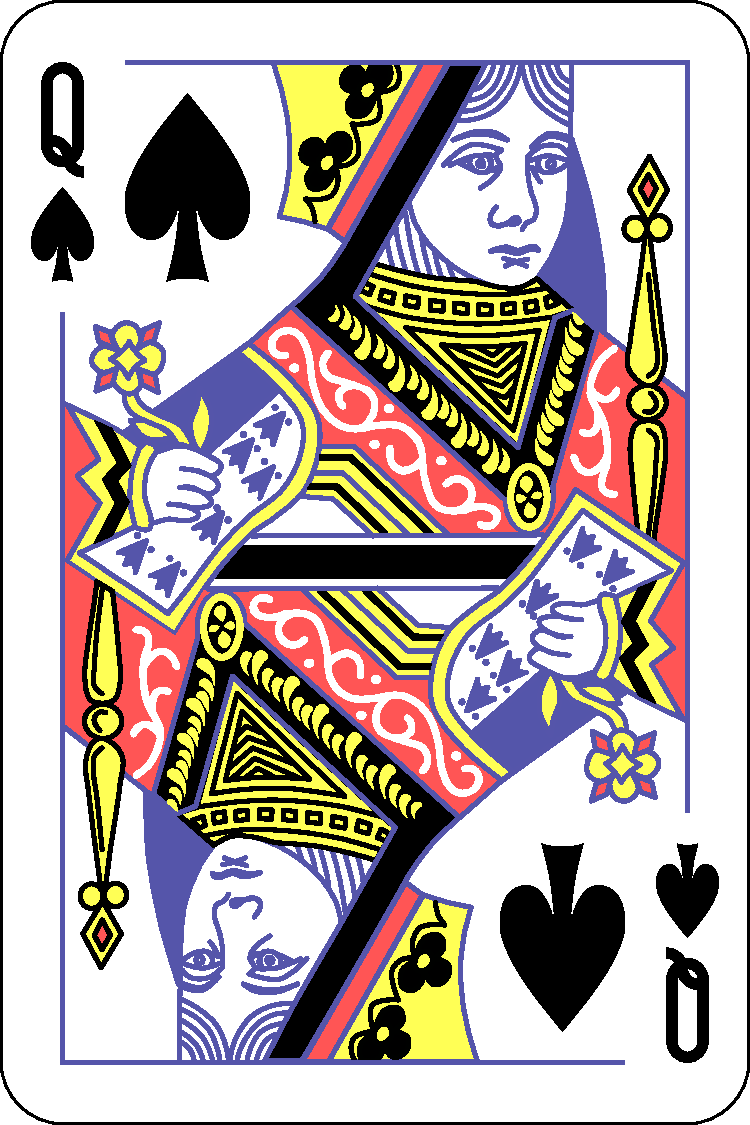
\includegraphics[width=.19\linewidth]{spade_q.pdf}
        \includegraphics[width=.19\linewidth]{spade_j.pdf}
        \includegraphics[width=.19\linewidth]{spade_10.pdf} 
        \caption{\label{fig:royal_straight_flush}皇家同花顺示例}
    \end{figure}
\end{itemize}
\subsection{术语}
发牌术语:
\begin{itemize}
    \item 底牌(Hole Cards):每位玩家在第一轮发牌时所得到的两张手牌。
    \item 翻牌(Flop):在第二轮发牌时,翻开的三张公共牌。
    \item 转牌(Turn):在第三轮发牌时,翻开的一张公共牌。
    \item 河牌(River):在最后一轮发牌时,翻开的最后一张公共牌。
下注术语:
\begin{itemize}
    \item 加注(Raise):在一个回合中,玩家可以对上一位玩家的下注加上更多的筹码。
    \item 跟住(Call):在一个回合中,玩家可以下注与上一位玩家的下注相同的筹码。
    \item 弃牌(Fold):在一个回合中,玩家可以放弃自己的牌,并退出这个回合。
    \item 全下(All-In):在一个回合中,玩家可以把自己所有的筹码都下注。
\end{itemize}
\end{itemize}
\subsection{例子}
\newpage
\section{概率工具}
概率是人类发明的处理不确定性的工具。
\section{概率在德扑中的应用}
\end{document}